%% This file was auto-generated by IPython.
%% Conversion from the original notebook file:
%% Exercise 11.ipynb
%%
\documentclass[11pt,english]{article}

%% This is the automatic preamble used by IPython.  Note that it does *not*
%% include a documentclass declaration. The documentclass is added at runtime
%% to the overall document.
\usepackage{fancyhdr}
\usepackage{amsmath}
\usepackage{amssymb}
\usepackage{graphicx}
\usepackage{ucs}
\usepackage[utf8x]{inputenc}

% needed for markdown enumerations to work
\usepackage{enumerate}

% Slightly bigger margins than the latex defaults
\usepackage{geometry}
\geometry{verbose,tmargin=3cm,bmargin=3cm,lmargin=2.5cm,rmargin=2.5cm}

% Define a few colors for use in code, links and cell shading
\usepackage{color}
\definecolor{orange}{cmyk}{0,0.4,0.8,0.2}
\definecolor{darkorange}{rgb}{.71,0.21,0.01}
\definecolor{darkgreen}{rgb}{.12,.54,.11}
\definecolor{myteal}{rgb}{.26, .44, .56}
\definecolor{gray}{gray}{0.45}
\definecolor{lightgray}{gray}{.95}
\definecolor{mediumgray}{gray}{.8}
\definecolor{inputbackground}{rgb}{.95, .95, .85}
\definecolor{outputbackground}{rgb}{.95, .95, .95}
\definecolor{traceback}{rgb}{1, .95, .95}

% Framed environments for code cells (inputs, outputs, errors, ...).  The
% various uses of \unskip (or not) at the end were fine-tuned by hand, so don't
% randomly change them unless you're sure of the effect it will have.
\usepackage{framed}

% remove extraneous vertical space in boxes
\setlength\fboxsep{0pt}

% codecell is the whole input+output set of blocks that a Code cell can
% generate.

% TODO: unfortunately, it seems that using a framed codecell environment breaks
% the ability of the frames inside of it to be broken across pages.  This
% causes at least the problem of having lots of empty space at the bottom of
% pages as new frames are moved to the next page, and if a single frame is too
% long to fit on a page, it will completely stop latex from compiling the
% document.  So unless we figure out a solution to this, we'll have to instead
% leave the codecell env. as empty.  I'm keeping the original codecell
% definition here (a thin vertical bar) for reference, in case we find a
% solution to the page break issue.

%% \newenvironment{codecell}{%
%%     \def\FrameCommand{\color{mediumgray} \vrule width 1pt \hspace{5pt}}%
%%    \MakeFramed{\vspace{-0.5em}}}
%%  {\unskip\endMakeFramed}

% For now, make this a no-op...
\newenvironment{codecell}{}

 \newenvironment{codeinput}{%
   \def\FrameCommand{\colorbox{inputbackground}}%
   \MakeFramed{\advance\hsize-\width \FrameRestore}}
 {\unskip\endMakeFramed}

\newenvironment{codeoutput}{%
   \def\FrameCommand{\colorbox{outputbackground}}%
   \vspace{-1.4em}
   \MakeFramed{\advance\hsize-\width \FrameRestore}}
 {\unskip\medskip\endMakeFramed}

\newenvironment{traceback}{%
   \def\FrameCommand{\colorbox{traceback}}%
   \MakeFramed{\advance\hsize-\width \FrameRestore}}
 {\endMakeFramed}

% Use and configure listings package for nicely formatted code
\usepackage{listingsutf8}
\lstset{
  language=python,
  inputencoding=utf8x,
  extendedchars=\true,
  aboveskip=\smallskipamount,
  belowskip=\smallskipamount,
  xleftmargin=2mm,
  breaklines=true,
  basicstyle=\small \ttfamily,
  showstringspaces=false,
  keywordstyle=\color{blue}\bfseries,
  commentstyle=\color{myteal},
  stringstyle=\color{darkgreen},
  identifierstyle=\color{darkorange},
  columns=fullflexible,  % tighter character kerning, like verb
}

% The hyperref package gives us a pdf with properly built
% internal navigation ('pdf bookmarks' for the table of contents,
% internal cross-reference links, web links for URLs, etc.)
\usepackage{hyperref}
\hypersetup{
  breaklinks=true,  % so long urls are correctly broken across lines
  colorlinks=true,
  urlcolor=blue,
  linkcolor=darkorange,
  citecolor=darkgreen,
  }

% hardcode size of all verbatim environments to be a bit smaller
\makeatletter
\g@addto@macro\@verbatim\small\topsep=0.5em\partopsep=0pt
\makeatother

% Prevent overflowing lines due to urls and other hard-to-break entities.
\sloppy

\newcommand{\HRule}{\rule{\linewidth}{0.5mm}}
\title{\bf Self Organizing Maps and Embedding}
\author{Xugang Zhou \\ Fangzhou Yang}
\pagestyle{fancy}
\lhead{{\bf Machine Intelligence 2 SS2013}}
\rhead{Exercise 11}
\renewcommand{\headrulewidth}{0.4pt}

\begin{document}
\begin{titlepage}
\begin{center}
\vfill
\textsc{\LARGE Machine Intelligence 2}\\[1.5cm]
\textsc{\Large Exercise 11}\\[0.5cm]

\HRule \\[0.4cm]
{\huge \bfseries Self Organizing Maps and Embedding}\\[0.4cm]
\HRule \\[1.5cm]
\begin{minipage}{0.4\textwidth}
\begin{flushleft} \large
\emph{Group Members:}\\
Xugang \textsc{Zhou}\\
Fangzhou \textsc{Yang}
\end{flushleft}
\end{minipage}
\begin{minipage}{0.4\textwidth}
\begin{flushright} \large
\emph{Tutor:} \\
Timm \textsc{Lochmann} \\
\end{flushright}
\end{minipage}
\vfill
{\large \today}\\
\end{center}
\end{titlepage}
\thispagestyle{fancy}

\section{1d Self-Organizing Map for 2d data}

\begin{codecell}
\begin{codeinput}
\begin{lstlisting}
#functions
def plotScatter(X,Y,title,c):
    fig = plt.figure()
    ax = fig.add_subplot(111)
    #ax.axis([-ran,ran,-ran,ran])
    ax.plot(X,Y,c+'.')
    ax.set_title(title)
    plt.show()
    
def plotW(X,Y,W,title,c):
    fig = plt.figure()
    ax = fig.add_subplot(111)
    #ax.axis([-ran,ran,-ran,ran])
    ax.plot(X,Y,c+'.')
    ax.plot(W[:,0],W[:,1],"rD")
    ax.plot(W[:,0],W[:,1],"r-")
    ax.set_title(title)
    plt.show()
\end{lstlisting}
\end{codeinput}
\end{codecell}
\begin{codecell}
\begin{codeinput}
\begin{lstlisting}
#data generator
random.seed(100)
X = random.uniform(0,2,1000)
Y = random.uniform(0,1,1000)
data = [[0 for j in range(2)] for i in range (1000)]
for i in range(1000):
    data[i][0] = X[i]
    data[i][1] = Y[i]
data = array(data)
plotScatter(X,Y,"Scatter Plot of Uniform Distribution","c")

\end{lstlisting}
\end{codeinput}
\begin{codeoutput}
\begin{center}
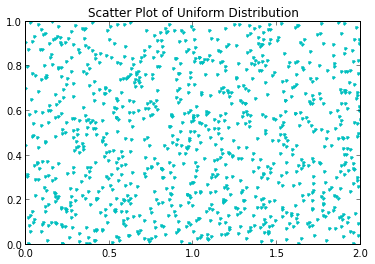
\includegraphics[width=0.7\textwidth]{Exercise_11_files/Exercise_11_fig_00.png}
\par
\end{center}
\end{codeoutput}
\end{codecell}
\begin{codecell}
\begin{codeinput}
\begin{lstlisting}
#init_W
def init_W(data,k):
    d = len(data[0])
    center = [0 for i in range (d)]
    for i in range(d):
        center[i] = sum(data[:,i])/len(data)
    random.seed(200)
    W = [[0 for j in range(d)] for i in range(k)]
    for i in range(k):
        for j in range(d):
            W[i][j] = center[j] + random.random() * 0.4 -0.2
    return W

#1d-SOM
def SOM_1d(data,k,W_init,xi,sigma):
    sigma0 = sigma
    xi0 = xi
    W = array(W_init)
    delta_W = array(W_init)
    d = len(data[0])
    size = len(data)
    
    flag = True
    alpha =0
    iteration = 0.
    while(flag):
        #choose the closest P
        for p in range (k):
            if (p==0):
                dis_min = distance(data[alpha],W[p])
                p_min = p
            else:
                dis = distance(data[alpha],W[p])
                if(dis<dis_min):
                    dis_min=dis
                    p_min = p
        #change prototypes
        for q in range (k):
            delta_W[q] = xi * h_qp([q],[p_min],sigma) * (data[alpha] - W[q])
        for i in range (k):
            W[i] = W[i] + delta_W[i]
        
        if(sigma<0.00000001):
            flag = False
            
        alpha = (alpha+1)%size
        iteration +=1
        if(iteration > size ):
            sigma = sigma * (size/iteration)
            xi = xi * (size/iteration)
        
    return W

def h_qp(w1,w2,sigma):
    sqsum = 0.
    for i in range (len(w1)):
        sqsum += (w1[i] - w2[i])**2
    #print sigma
    tmp = -sqsum/(2* sigma**2)
    return math.exp(tmp)
    
   
def distance(x,w):
    tmpsum = 0.
    for i in range (len(x)):
        tmpsum += (x[i] - w[i])**2
    dis = math.sqrt(tmpsum)
    return dis
\end{lstlisting}
\end{codeinput}
\end{codecell}
\begin{codecell}
\begin{codeinput}
\begin{lstlisting}
W = init_W(data,4)
plotW(X,Y,array(W),"k=4 init","c")
W_final = SOM_1d(data,4,W,0.002,1.0)
plotW(X,Y,W_final,"k=4 result","c")
\end{lstlisting}
\end{codeinput}
\begin{codeoutput}
\begin{center}
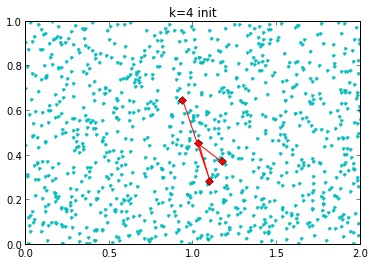
\includegraphics[width=0.7\textwidth]{Exercise_11_files/Exercise_11_fig_01.png}
\par
\end{center}
\begin{center}
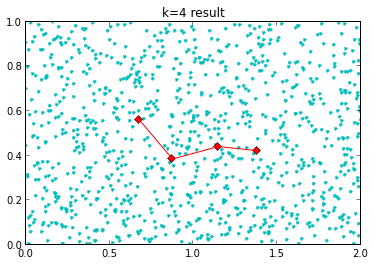
\includegraphics[width=0.7\textwidth]{Exercise_11_files/Exercise_11_fig_02.png}
\par
\end{center}
\end{codeoutput}
\end{codecell}
\begin{codecell}
\begin{codeinput}
\begin{lstlisting}
W = init_W(data,8)
plotW(X,Y,array(W),"k=8 init","c")
W_final = SOM_1d(data,8,W,0.004,2.)
plotW(X,Y,W_final,"k=8 result","c")
\end{lstlisting}
\end{codeinput}
\begin{codeoutput}
\begin{center}
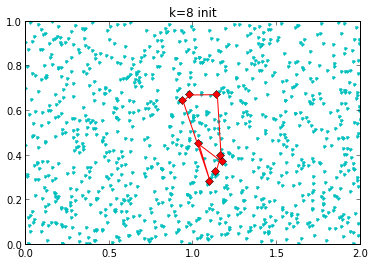
\includegraphics[width=0.7\textwidth]{Exercise_11_files/Exercise_11_fig_03.png}
\par
\end{center}
\begin{center}
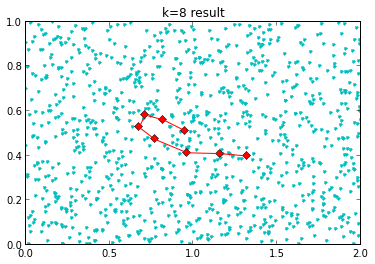
\includegraphics[width=0.7\textwidth]{Exercise_11_files/Exercise_11_fig_04.png}
\par
\end{center}
\end{codeoutput}
\end{codecell}
\begin{codecell}
\begin{codeinput}
\begin{lstlisting}
W = init_W(data,16)
plotW(X,Y,array(W),"k=16 init","c")
W_final = SOM_1d(data,16,W,0.008,4.)
plotW(X,Y,W_final,"k=16 result","c")
\end{lstlisting}
\end{codeinput}
\begin{codeoutput}
\begin{center}
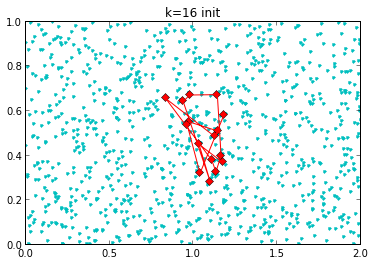
\includegraphics[width=0.7\textwidth]{Exercise_11_files/Exercise_11_fig_05.png}
\par
\end{center}
\begin{center}
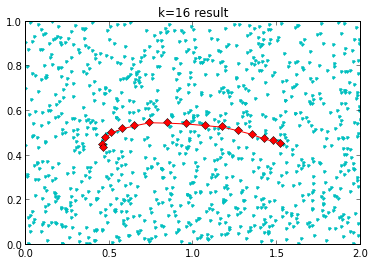
\includegraphics[width=0.7\textwidth]{Exercise_11_files/Exercise_11_fig_06.png}
\par
\end{center}
\end{codeoutput}
\end{codecell}
\begin{codecell}
\begin{codeinput}
\begin{lstlisting}
W = init_W(data,32)
plotW(X,Y,array(W),"k=32 init","c")
W_final = SOM_1d(data,32,W,0.01,8.)
plotW(X,Y,W_final,"k=16 result","c")
\end{lstlisting}
\end{codeinput}
\begin{codeoutput}
\begin{center}
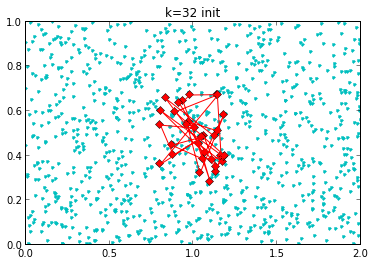
\includegraphics[width=0.7\textwidth]{Exercise_11_files/Exercise_11_fig_07.png}
\par
\end{center}
\begin{center}
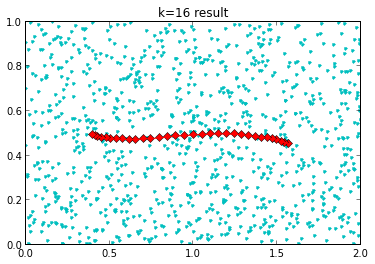
\includegraphics[width=0.7\textwidth]{Exercise_11_files/Exercise_11_fig_08.png}
\par
\end{center}
\end{codeoutput}
\end{codecell}
\begin{codecell}
\begin{codeinput}
\begin{lstlisting}
W = init_W(data,64)
plotW(X,Y,array(W),"k=64 init","c")
W_final = SOM_1d(data,64,W,0.012,16.)
plotW(X,Y,W_final,"k=64 result","c")
\end{lstlisting}
\end{codeinput}
\begin{codeoutput}
\begin{center}
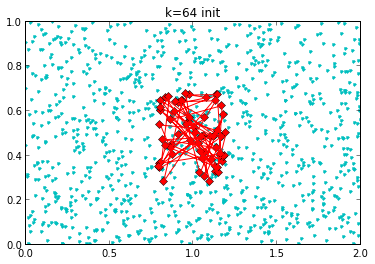
\includegraphics[width=0.7\textwidth]{Exercise_11_files/Exercise_11_fig_09.png}
\par
\end{center}
\begin{center}
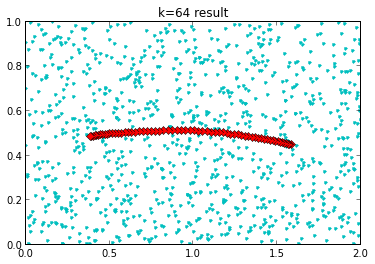
\includegraphics[width=0.7\textwidth]{Exercise_11_files/Exercise_11_fig_10.png}
\par
\end{center}
\end{codeoutput}
\end{codecell}
\section{1d Self-Organizing Maps for 3d data}

\begin{codecell}
\begin{codeinput}
\begin{lstlisting}
from mpl_toolkits.mplot3d import Axes3D
def plot3dScatter(X,Y,Z,title,c):
    fig = plt.figure()
    ax = Axes3D(fig)
    ax.plot(X,Y,Z,c)
    ax.set_title(title)
    plt.show()
\end{lstlisting}
\end{codeinput}
\end{codecell}
\begin{codecell}
\begin{codeinput}
\begin{lstlisting}
#read data
spiral = loadtxt("spiral.csv",skiprows=1,delimiter=",",usecols=(1,2,3))
plot3dScatter(spiral[:,0],spiral[:,1],spiral[:,2],"scatter plot of spiral","c.")
\end{lstlisting}
\end{codeinput}
\begin{codeoutput}
\begin{center}
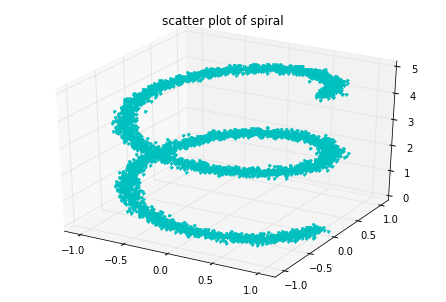
\includegraphics[width=0.7\textwidth]{Exercise_11_files/Exercise_11_fig_11.png}
\par
\end{center}
\end{codeoutput}
\end{codecell}
\begin{codecell}
\begin{codeinput}
\begin{lstlisting}
#init_W
def init_W_3d(data,k):
    
    W = [ [0,0, float(i)*5/k ]for i in range (k)]
    
    return W

def plotW_3d(data,W,title,c):
    fig = plt.figure()
    ax = Axes3D(fig)
    ax.plot(data[:,0],data[:,1],data[:,2],c+'.')
    ax.plot(W[:,0],W[:,1],W[:,2],"rD")
    ax.plot(W[:,0],W[:,1],W[:,2],"r-")
    ax.set_title(title)
    plt.show()
\end{lstlisting}
\end{codeinput}
\end{codecell}
\begin{codecell}
\begin{codeinput}
\begin{lstlisting}
W = init_W_3d(spiral,16)
plotW_3d(spiral,array(W),"k=16 init","c")
W_final = SOM_1d(spiral,16,W,0.002,2.)
plotW_3d(spiral,W_final,"k=16 result","c")
\end{lstlisting}
\end{codeinput}
\begin{codeoutput}
\begin{center}
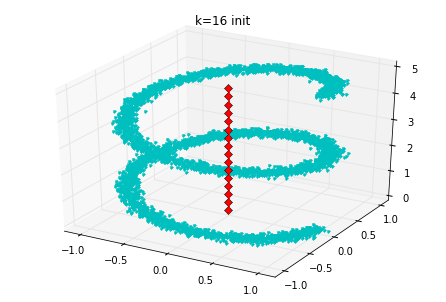
\includegraphics[width=0.7\textwidth]{Exercise_11_files/Exercise_11_fig_12.png}
\par
\end{center}
\begin{center}
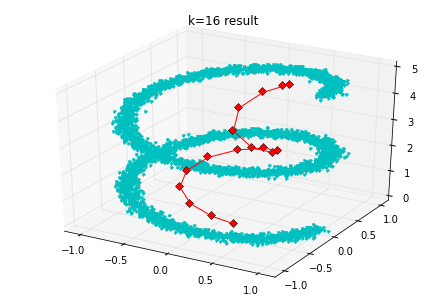
\includegraphics[width=0.7\textwidth]{Exercise_11_files/Exercise_11_fig_13.png}
\par
\end{center}
\end{codeoutput}
\end{codecell}
\begin{codecell}
\begin{codeinput}
\begin{lstlisting}
W = init_W_3d(spiral,32)
plotW_3d(spiral,array(W),"k=32 init","c")
W_final = SOM_1d(spiral,32,W,0.002,4.)
plotW_3d(spiral,W_final,"k=32 result","c")
\end{lstlisting}
\end{codeinput}
\begin{codeoutput}
\begin{center}
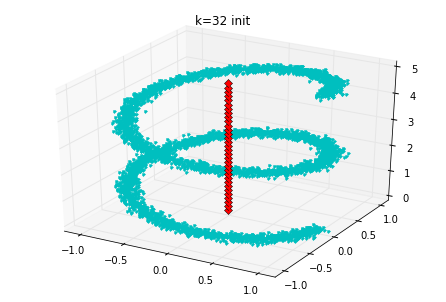
\includegraphics[width=0.7\textwidth]{Exercise_11_files/Exercise_11_fig_14.png}
\par
\end{center}
\begin{center}
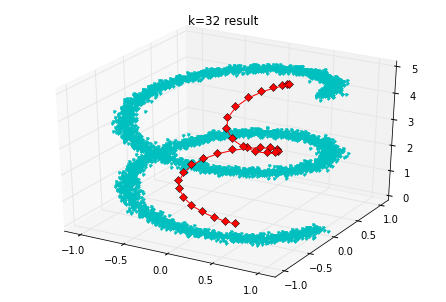
\includegraphics[width=0.7\textwidth]{Exercise_11_files/Exercise_11_fig_15.png}
\par
\end{center}
\end{codeoutput}
\end{codecell}
\begin{codecell}
\begin{codeinput}
\begin{lstlisting}
W = init_W_3d(spiral,64)
plotW_3d(spiral,array(W),"k=64 init","c")
W_final = SOM_1d(spiral,64,W,0.002,8.)
plotW_3d(spiral,W_final,"k=64 result","c")
\end{lstlisting}
\end{codeinput}
\begin{codeoutput}
\begin{center}
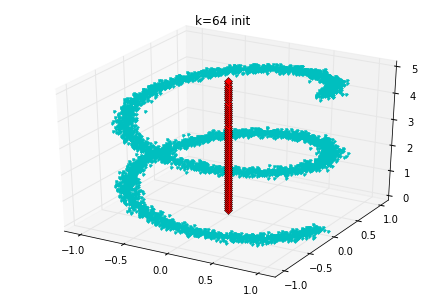
\includegraphics[width=0.7\textwidth]{Exercise_11_files/Exercise_11_fig_16.png}
\par
\end{center}
\begin{center}
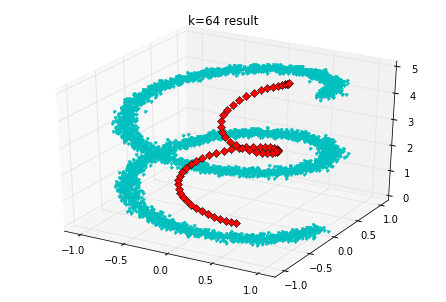
\includegraphics[width=0.7\textwidth]{Exercise_11_files/Exercise_11_fig_17.png}
\par
\end{center}
\end{codeoutput}
\end{codecell}
\begin{codecell}
\begin{codeinput}
\begin{lstlisting}
W = init_W_3d(spiral,128)
plotW_3d(spiral,array(W),"k=128 init","c")
W_final = SOM_1d(spiral,128,W,0.002,16.)
plotW_3d(spiral,W_final,"k=128 result","c")
\end{lstlisting}
\end{codeinput}
\begin{codeoutput}
\begin{center}
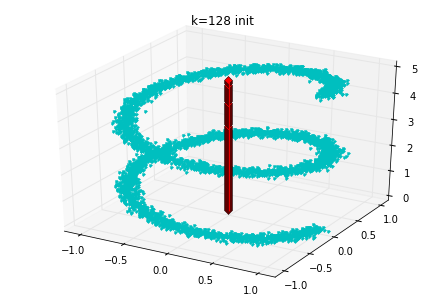
\includegraphics[width=0.7\textwidth]{Exercise_11_files/Exercise_11_fig_18.png}
\par
\end{center}
\begin{center}
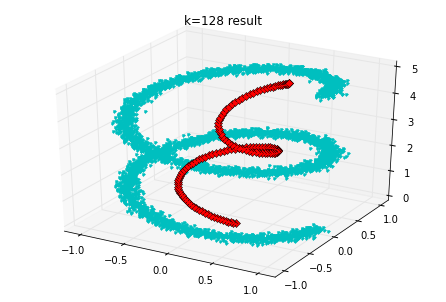
\includegraphics[width=0.7\textwidth]{Exercise_11_files/Exercise_11_fig_19.png}
\par
\end{center}
\end{codeoutput}
\end{codecell}
\section{2d Self-Organizing Maps for 3d data}

\begin{codecell}
\begin{codeinput}
\begin{lstlisting}
#2d-SOM
def SOM_2d(data,k,W_init,xi,sigma):
    W = array(W_init)
    delta_W = array(W_init)
    d = len(data[0])
    size = len(data)
    
    flag = True
    alpha =0
    iteration = 0.
    while(flag):
        #choose the closest P
        for pi in range (k):
            for pj in range (k):
                if (pi==0 and pj==0):
                    dis_min = distance(data[alpha],W[pi][pj])
                    pi_min = pi
                    pj_min = pj
            else:
                dis = distance(data[alpha],W[pi][pj])
                if(dis < dis_min):
                    dis_min = dis
                    pi_min = pi
                    pj_min = pj
        for qi in range (k):
            for qj in range (k):
                delta_W[qi][qj] = xi * h_qp([qi,qj],[pi_min,pj_min],sigma) * (data[alpha] - W[qi][qj])
                
        for i in range (k):
            for j in range (k):
                W[i][j] = W[i][j] + delta_W[i][j]
        
        if(sigma<0.0000000000001):
            flag = False
            break;
        alpha = (alpha+1)%size
        iteration +=1
        if(iteration > size):
            sigma = sigma * (size/iteration)
            #xi = xi * (size/iteration)
        
    return W
\end{lstlisting}
\end{codeinput}
\end{codecell}
\begin{codecell}
\begin{codeinput}
\begin{lstlisting}
#read data
bowl = loadtxt("bowl.csv",skiprows=1,delimiter=",",usecols=(1,2,3))
plot3dScatter(bowl[:,0],bowl[:,1],bowl[:,2],"scatter plot of bowl","c.")
\end{lstlisting}
\end{codeinput}
\begin{codeoutput}
\begin{center}
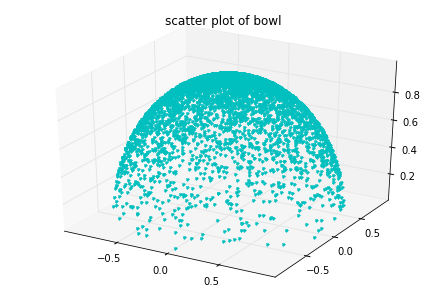
\includegraphics[width=0.7\textwidth]{Exercise_11_files/Exercise_11_fig_20.png}
\par
\end{center}
\end{codeoutput}
\end{codecell}
\begin{codecell}
\begin{codeinput}
\begin{lstlisting}
#init_W
def init_W_bowl(data,k):
    
    W = [[ [float(i+1)/(k+1)*2-1.,float(j+1)/(k+1)*2-1., 0.4 ]for j in range (k)]for i in range (k)]
    
    return W

def plotW_3d_bowl(data,W,title,c):
    fig = plt.figure()
    ax = Axes3D(fig)
    ax.plot(data[:,0],data[:,1],data[:,2],c+'.')
    k = len(W)
    for i in range (k):
        ax.plot(W[i,:,0],W[i,:,1],W[i,:,2],"rD")
        ax.plot(W[i,:,0],W[i,:,1],W[i,:,2],"r-")
    for i in range (k):
        ax.plot(W[:,i,0],W[:,i,1],W[:,i,2],"rD")
        ax.plot(W[:,i,0],W[:,i,1],W[:,i,2],"r-")
    ax.set_title(title)
    plt.show()
    
def plotW_map(data,W):
    k = len(W)
    size = len(data)
    alpha = 0
    C = [[0 for i in range(k)] for j in range (k)]
    for alpha in range (size):
        #choose the closest P
        for pi in range (k):
            for pj in range (k):
                if (pi==0 and pj==0):
                    dis_min = distance(data[alpha],W[pi][pj])
                    pi_min = pi
                    pj_min = pj
                else:
                    dis = distance(data[alpha],W[pi][pj])
                    if(dis < dis_min):
                        dis_min = dis
                        pi_min = pi
                        pj_min = pj
        C[pi_min][pj_min] += 1
               
    plt.title("2d_Map of Dataset_Bowl")
    plt.imshow(C,interpolation="nearest",extent=[1,k,1,k])
    plt.colorbar()
    plt.show()
    
\end{lstlisting}
\end{codeinput}
\end{codecell}
\begin{codecell}
\begin{codeinput}
\begin{lstlisting}
W = init_W_bowl(bowl,8)
plotW_3d_bowl(bowl,array(W),"k=8 init","c")
W_final1 = SOM_2d(bowl,8,W,0.0002,4.)
plotW_3d_bowl(bowl,W_final1,"k=8 result","c")
\end{lstlisting}
\end{codeinput}
\begin{codeoutput}
\begin{center}
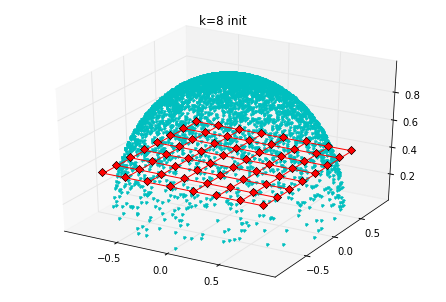
\includegraphics[width=0.7\textwidth]{Exercise_11_files/Exercise_11_fig_21.png}
\par
\end{center}
\begin{center}
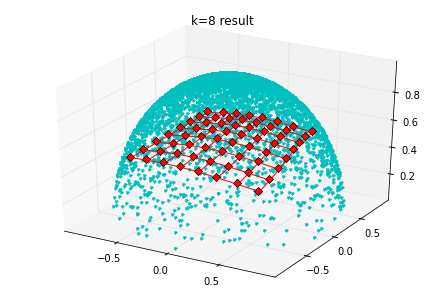
\includegraphics[width=0.7\textwidth]{Exercise_11_files/Exercise_11_fig_22.png}
\par
\end{center}
\end{codeoutput}
\end{codecell}
\begin{codecell}
\begin{codeinput}
\begin{lstlisting}
plotW_map(bowl,W_final1)
\end{lstlisting}
\end{codeinput}
\begin{codeoutput}
\begin{center}
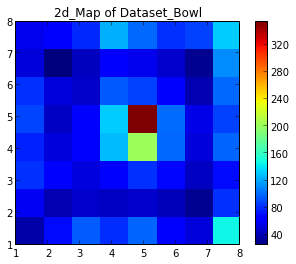
\includegraphics[width=0.7\textwidth]{Exercise_11_files/Exercise_11_fig_23.png}
\par
\end{center}
\end{codeoutput}
\end{codecell}
\begin{codecell}
\begin{codeinput}
\begin{lstlisting}
W = init_W_bowl(bowl,16)
plotW_3d_bowl(bowl,array(W),"k=16 init","c")
W_final2 = SOM_2d(bowl,16,W,0.0002,8.)
plotW_3d_bowl(bowl,W_final2,"k=16 result","c")
\end{lstlisting}
\end{codeinput}
\begin{codeoutput}
\begin{center}
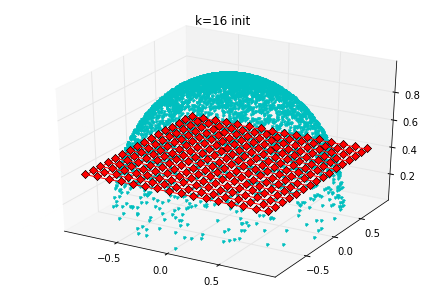
\includegraphics[width=0.7\textwidth]{Exercise_11_files/Exercise_11_fig_24.png}
\par
\end{center}
\begin{center}
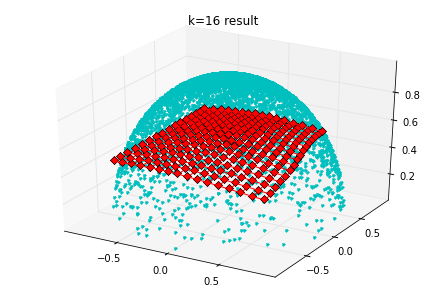
\includegraphics[width=0.7\textwidth]{Exercise_11_files/Exercise_11_fig_25.png}
\par
\end{center}
\end{codeoutput}
\end{codecell}
\begin{codecell}
\begin{codeinput}
\begin{lstlisting}
plotW_map(bowl,W_final2)
\end{lstlisting}
\end{codeinput}
\begin{codeoutput}
\begin{center}
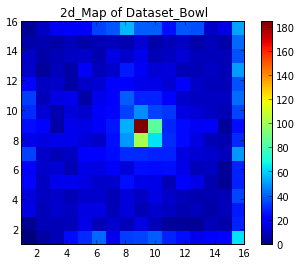
\includegraphics[width=0.7\textwidth]{Exercise_11_files/Exercise_11_fig_26.png}
\par
\end{center}
\end{codeoutput}
\end{codecell}
\begin{codecell}
\begin{codeinput}
\begin{lstlisting}
W = init_W_bowl(bowl,32)
plotW_3d_bowl(bowl,array(W),"k=32 init","c")
W_final3 = SOM_2d(bowl,32,W,0.0002,16.)
plotW_3d_bowl(bowl,W_final3,"k=32 result","c")
\end{lstlisting}
\end{codeinput}
\begin{codeoutput}
\begin{center}
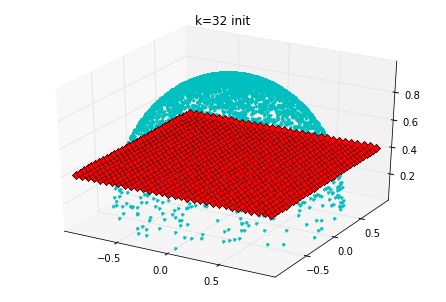
\includegraphics[width=0.7\textwidth]{Exercise_11_files/Exercise_11_fig_27.png}
\par
\end{center}
\begin{center}
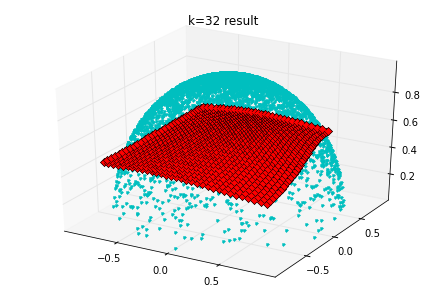
\includegraphics[width=0.7\textwidth]{Exercise_11_files/Exercise_11_fig_28.png}
\par
\end{center}
\end{codeoutput}
\end{codecell}
\begin{codecell}
\begin{codeinput}
\begin{lstlisting}
plotW_map(bowl,W_final3)
\end{lstlisting}
\end{codeinput}
\begin{codeoutput}
\begin{center}
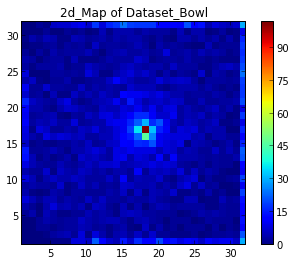
\includegraphics[width=0.7\textwidth]{Exercise_11_files/Exercise_11_fig_29.png}
\par
\end{center}
\end{codeoutput}
\end{codecell}

\end{document}
